\section{Nombre: Fantasma rojo}   \label{per:fantasmaR}
\subsection{Descripción:}
Este enemigo nace de las almas que no quedaron varadas en los niveles del Mictlán al no poder terminar los desafíos. Tiene la forma de un cráneo, en los orificios de los ojos del cráneo se puede ver un brillo espectral. El cráneo está decorado con diferentes patrones de color rojo y verde petróleo en la zona superior del cráneo, la frente, los ojos y la boca. De la parte trasera del cráneo sale fuego cuya paleta de colores es un degradado de rojo y naranja, siendo el rojo el predominante. 
\subsection{Status:}
Enemigo.
\subsection{Imagen}
Ver figura \ref{fig:fantasmaR}.
\begin{figure}
	\centering
	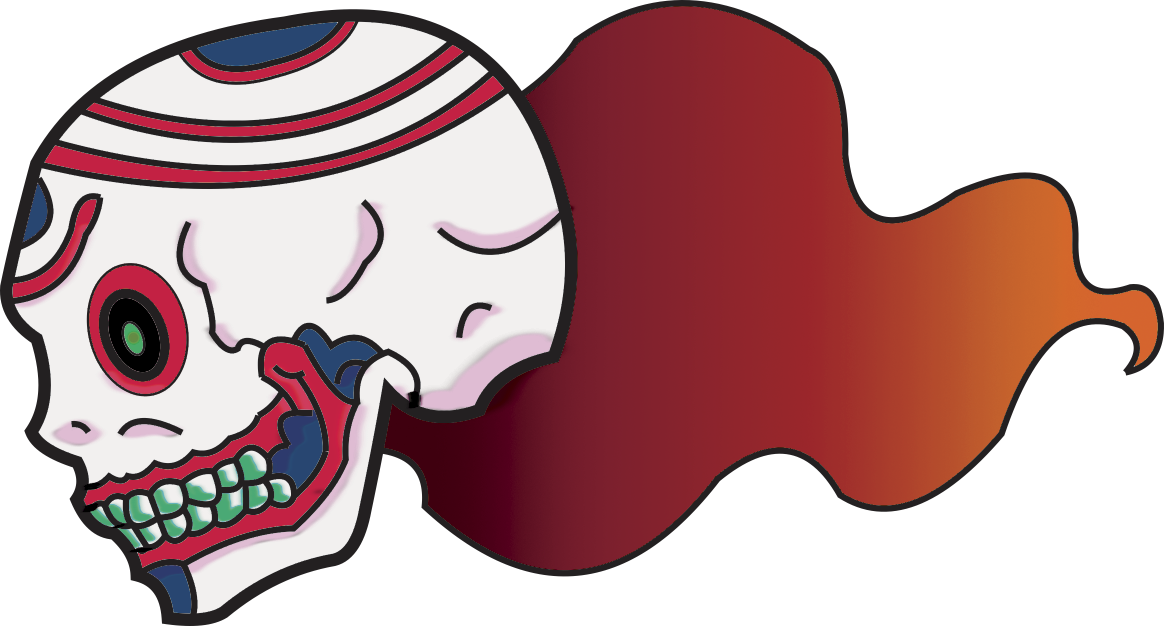
\includegraphics[height=0.2 \textheight]{Imagenes/fantasmaRojo}
	\caption{Fantasma rojo.}
	\label{fig:fantasmaR}
\end{figure} 
\subsection{Encuentro:}
Enemigo de los niveles 2, 3, 6, 7, 8 y 9. (ver apartados \ref{Nivel:Niv02}, \ref{Nivel:Niv03})
\subsection{Habilidades:}
\begin{itemize}
	\item Disparo rojo. Ver \ref{hab.disparoR}.
\end{itemize}
\subsection{Patrón de ataque:}
El enemigo realizara un recorrido vertical del punto A al B y del B al A de manera cíclica mientras ejecuta la habilidad de disparo rojo.
\subsection{Bloques de animación:}
		\begin{itemize}
			\item Animación fuego.
			\item Animación disparo.
		\end{itemize}